\documentclass[12pt]{article}
\date{November 22, 2023}
\usepackage{pgf-pie}
\usepackage{pgfplots}
\usepackage{pgfplotstable}
\usetikzlibrary{patterns}
\usepackage[section]{placeins}
\usepackage[utf8]{inputenc}

\begin{document}


\clearpage{}
\section{Does the website appear easy to navigate?}

\label{sec:1}


\begin{figure}[h!]
    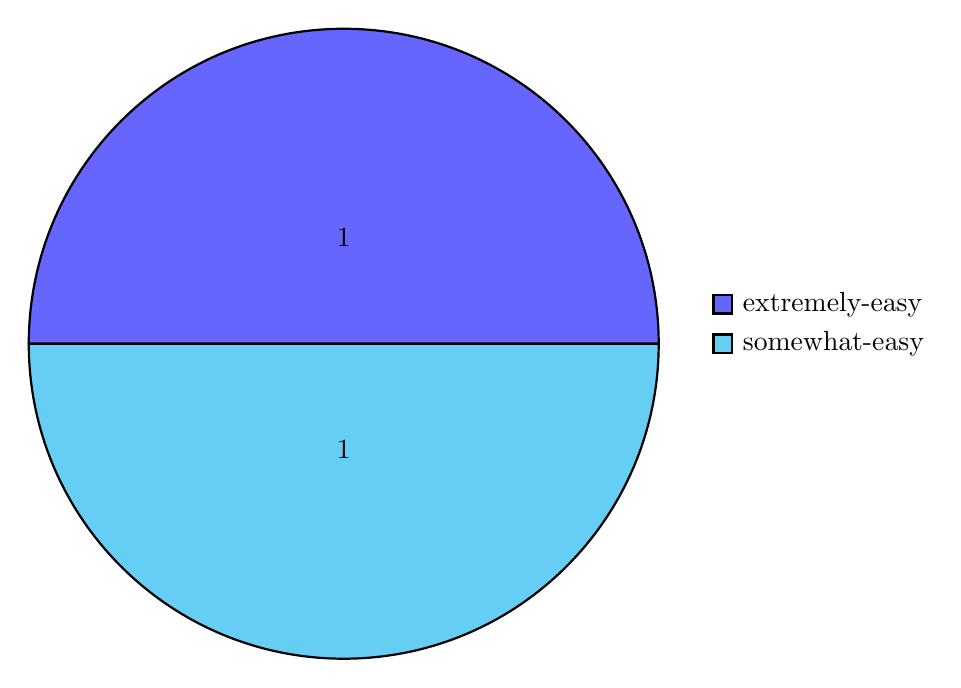
\begin{tikzpicture}
        \pie[radius=4,sum=auto,text=legend]{
            1/extremely-easy,
            1/somewhat-easy
        }
    \end{tikzpicture}
    \caption{\label{figure:q1-1}Repartition of answers for the question 'Does the website appear easy to navigate?'.}
\end{figure}



\clearpage{}
\section{Does the website have all the features and functionalities you expected?}

\label{sec:2}


\begin{figure}[h!]
    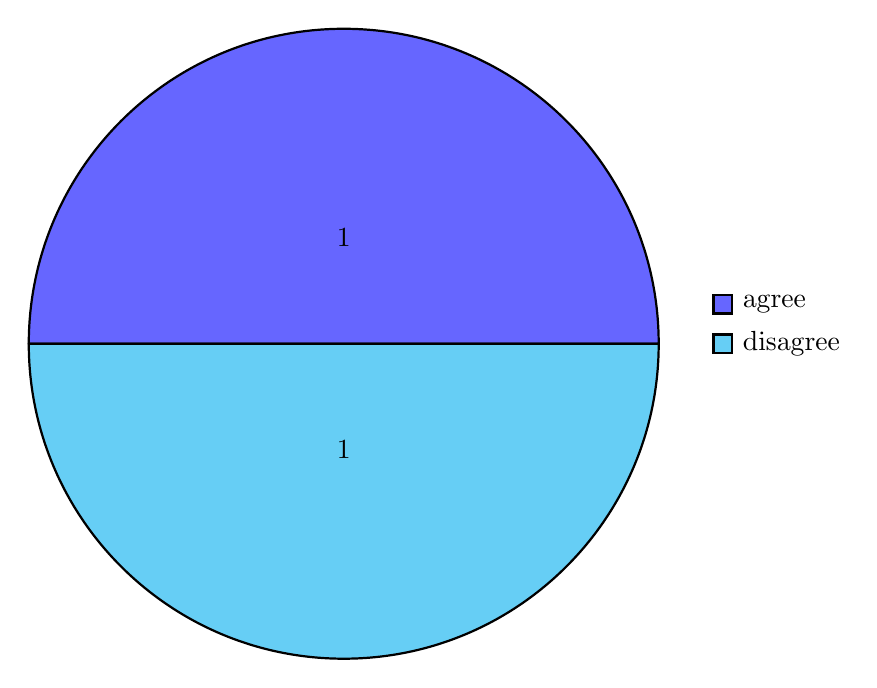
\begin{tikzpicture}
        \pie[radius=4,sum=auto,text=legend]{
            1/agree,
            1/disagree
        }
    \end{tikzpicture}
    \caption{\label{figure:q2-1}Repartition of answers for the question 'Does the website have all the features and functionalities you expected?'.}
\end{figure}



\clearpage{}
\section{Are you satisfied with how the website handled the scholarship application submission?}

\label{sec:3}


\begin{figure}[h!]
    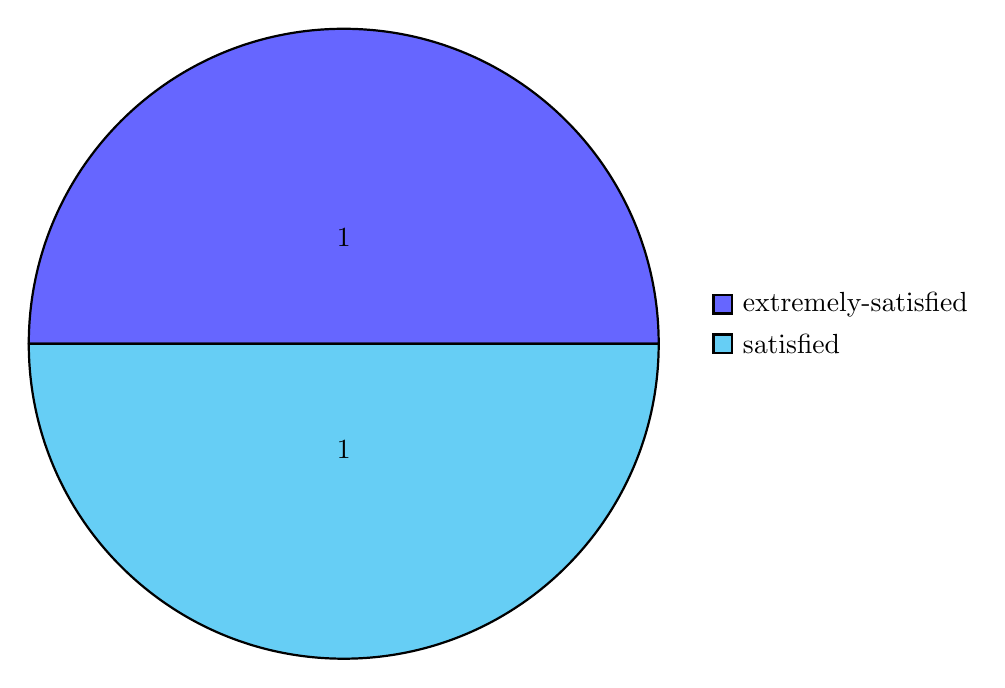
\begin{tikzpicture}
        \pie[radius=4,sum=auto,text=legend]{
            1/extremely-satisfied,
            1/satisfied
        }
    \end{tikzpicture}
    \caption{\label{figure:q3-1}Repartition of answers for the question 'Are you satisfied with how the website handled the scholarship application submission?'.}
\end{figure}



\clearpage{}
\section{How satisfied are you with the reliability of this website?}

\label{sec:4}


\begin{figure}[h!]
    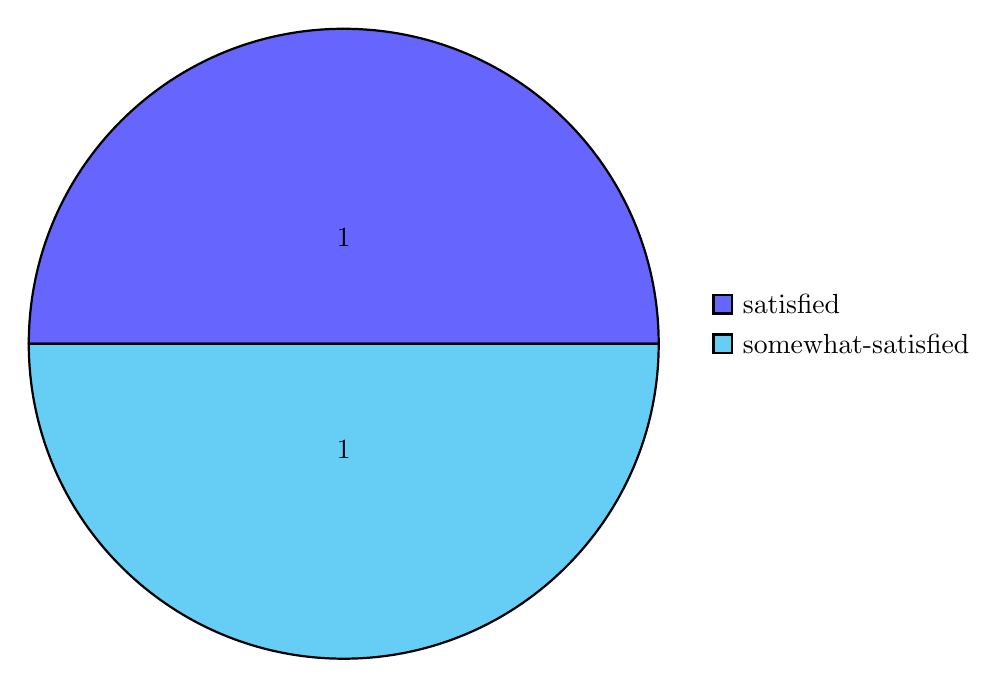
\begin{tikzpicture}
        \pie[radius=4,sum=auto,text=legend]{
            1/satisfied,
            1/somewhat-satisfied
        }
    \end{tikzpicture}
    \caption{\label{figure:q4-1}Repartition of answers for the question 'How satisfied are you with the reliability of this website?'.}
\end{figure}



\clearpage{}
\section{What do you like the least about the website?}

\label{sec:5}


\begin{figure}[h!]
    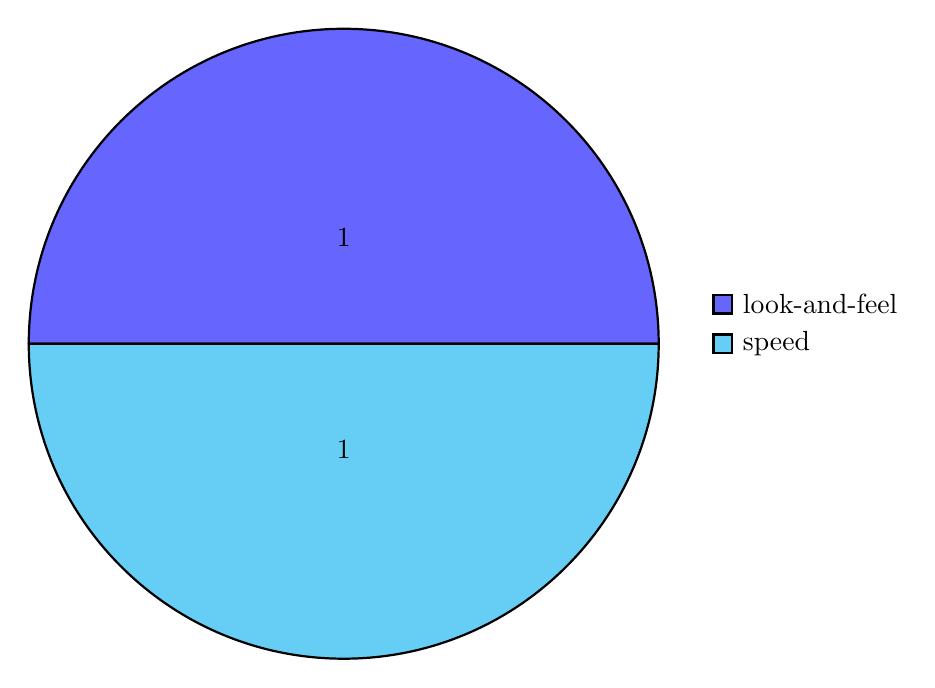
\begin{tikzpicture}
        \pie[radius=4,sum=auto,text=legend]{
            1/look-and-feel,
            1/speed
        }
    \end{tikzpicture}
    \caption{\label{figure:q5-1}Repartition of answers for the question 'What do you like the least about the website?'.}
\end{figure}



\clearpage{}
\section{Overall, how would you rate the quality of the system?}

\label{sec:6}


\begin{figure}[h!]
    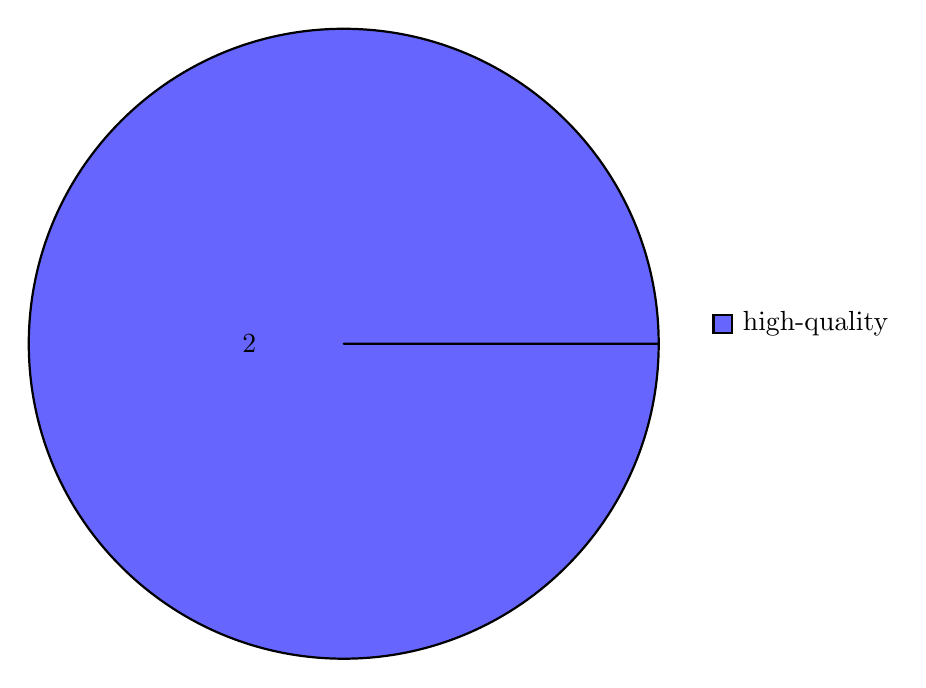
\begin{tikzpicture}
        \pie[radius=4,sum=auto,text=legend]{
            2/high-quality
        }
    \end{tikzpicture}
    \caption{\label{figure:q6-1}Repartition of answers for the question 'Overall, how would you rate the quality of the system?'.}
\end{figure}



\end{document}
